\documentclass[10pt]{article}
\usepackage[T1]{fontenc}
\usepackage{lmodern,amsmath,amssymb,graphicx,hyperref,array}
\usepackage[margin=.78in]{geometry}
\setlength{\parindent}{0pt}\setlength{\parskip}{6pt}
\begin{document}
\begin{center}{\Large Deriving the branch and translated order}\\[3pt]
23 November 2026 --- distinct local unsigned proof components\end{center}
\textbf{An actual curve branch.} Over a field $K$, assume
$y^2=f(x)$, $2\ne0$, $y\ne0$. Define the actual series
$g=f\bigl(Cx+T\bigr)$ by polynomial evaluation through $C:K\to K[[T]]$.
Its constant coefficient is $f(x)$. The separately audited generic
Hensel application derives
\[
 \exists s,\ [T^0]s=y,\ s^2=g;
 \qquad \exists u,\ (Cy+Tu)^2=g.
\]
No favorable branch or Henselian instance is supplied. The generic
lemma works over any commutative ring when $2y$ is a unit. It provides
existence, not a finite-time coefficient routine or expected cost
(PCC-20261123-b4e7e9, b832ad, bc413b) [pcc:unverified].

\textbf{Actual translated order.} Let $p\in K[X][Y]$ have the study's
actual full mixed multiplicity $r$ at $(x,y)$. Form explicitly
\[
 q=\operatorname{map}(\mathrm{Taylor}_y)
 \left(\operatorname{swap}\bigl(\operatorname{map}(\mathrm{Taylor}_x)p\bigr)\right).
\]
The exported mixed-coefficient identity, coefficient-map law and
public Taylor value equation derive $[U^iV^j]q=0$ when $j+i<r$.
A separate generic semiring theorem then gives
\[
 T^r\mid \operatorname{TwoEval}(C,Tu,T,q),
 \quad\operatorname{TwoEval}(h,a,b,q)=q.\operatorname{eval}_2
       (\operatorname{eval}_2\mathrm{Hom}(h,a),b).
\]
This concerns the actual explicit translation composition for every
natural $r$, including zero. No evaluated-divisibility witness is
assumed (PCC-20261123-d23220, d133b7, f093a1) [pcc:unverified].

\begin{center}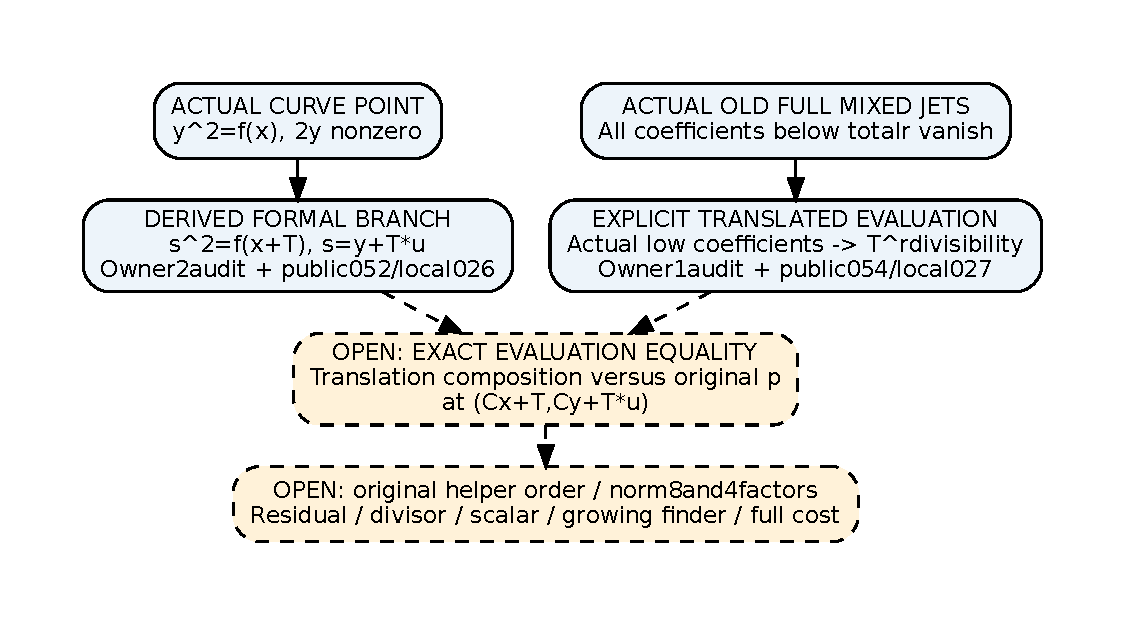
\includegraphics[width=.90\linewidth,height=.41\textheight,keepaspectratio]{branch-dependencies-001.pdf}\end{center}
\textbf{The remaining semantic arrow is explicit.}
The equality of this translated evaluation with original $p$ at
$(Cx+T,Cy+Tu)$ still needs a proof. Consequently actual original-helper
$T^4$, paired norm order eight, target order four, residual degree and
useful divisor/scalar relations are not inferred from these components.
\newpage
\begin{center}{\Large Proof map, checks and next test}\end{center}
\textbf{Primary declarations.} Namespace prefix \texttt{Orientation}:
\begin{itemize}
\item \texttt{ActualFormalBranch.translatedCurve\_constantCoeff};
\item \texttt{ActualFormalBranch.actual\_branch\_exists};
\item \texttt{ActualFormalBranch.actual\_branch\_linear\_tail};
\item \texttt{ActualJetOrder.actual\_explicit\_shifted\_order}.
\end{itemize}
Source 052, build 055, receipt 026 accepts three new statements, 132 total.
Source 054, build 057, receipt 027 accepts one more, 133 total. Each exits zero
without warnings; all printed dependencies are standard. The prior
129 statements and nonzero cubic norm of degree at most 30 retain their
own exact source and evidence. All data are unsigned, outside shared
Transport53/57 audit/fresh (PCC-20261123-b4e7e9 and d23220)
[pcc:unverified].

\textbf{Separate generic owner modules.}
\texttt{CryptoLean.PowerSeriesSquareRoot}: two theorems,
focused build and existing audit two passed, zero extra trusted;
local commit \texttt{b3ce082}.
\texttt{CryptoLean.PolynomialBivariateOrder}: one theorem,
focused build and existing audit one passed, zero extra trusted;
local commit \texttt{70fe5fc}.
The latter expands actual finite coefficient sums. A low-total term
is zero; every other term contains $a^ib^j$ divisible by
$d^{i+j}$ and hence by $d^r$. No domain or positive-$r$ assumption is
needed. Existing Hensel, Taylor and divisibility algebra is reused,
with no arithmetic novelty claim [pcc:unverified].

\textbf{Inputs and preservation.}
Pinned Lean4.35.0, Mathlib
\texttt{cfc55fc58714a59dc06e6e79edc6d1d95140d3c2},
exact owner source/compiled inputs and separate50/55-file namespace
overlays are recorded. Old cached binaries are not replaced;
manifests, umbrella, gates, trust and CI are unchanged.
No whole-project/fresh or signed standing is inferred.
The generic reports are separately editable and inspected; all old
norm/noncurve reports and every immutable snapshot remain exact
[pcc:unverified].

\textbf{Failures retained.}
Root-owner source001 rejected numeric cast forms; build002 used a
wrong hash path and checked no theorem. Source002/build003 still
needed a public constant-coefficient numeric equation;003/build004
passed. Order-owner source001 parsed no-space inequality notation as
an initial-segment symbol;002fixed only spacing.
Primary053/build056 attempted to use imported nonexposed definitions.
Accepted054explicitly changes representation to the actual translation
composition, bound by the already exported coefficient equation.
It does not assert an unproved equality with the old opaque object.
No private-body import, instance/transparency or resource/trust
change was used. All failed source/raw/exit/precall bytes are retained.

\textbf{Next discriminating identity.}
For an actual ring homomorphism $h:R\to A$, test
\[
 \operatorname{TwoEval}(h,a,b,q)=
 \operatorname{TwoEval}(h,b+h(x),a+h(y),p).
\]
Use public Taylor-composition, swap-monomial, coefficient-map and
ring-homomorphism equations; a missing generic interface belongs in
the owner first. Then bind the actual branch and original helper,
prove norm factors, and inspect divisor/group cancellation before
claiming useful relations. Residual splitting, factor-base membership,
known logarithms, growing public finding, retry and full expected bit
cost remain open. Protected remote ledger divergence blocks push;
no history reconciliation, signing or gate bypass was attempted [pcc:unverified].
\end{document}
